\section{Linearen Regression}
\begin{frame}{Lineare Regression}
    Die Idee hinter der Linearen Regression ist, dass zwischen zwei Variablen in einem Datensatz ein Zusammenhang existiert, den man bis auf einen Fehler durch eine lineare Gleichung darstellen kann.

    \only<1>{
    \begin{figure}
        \centering
        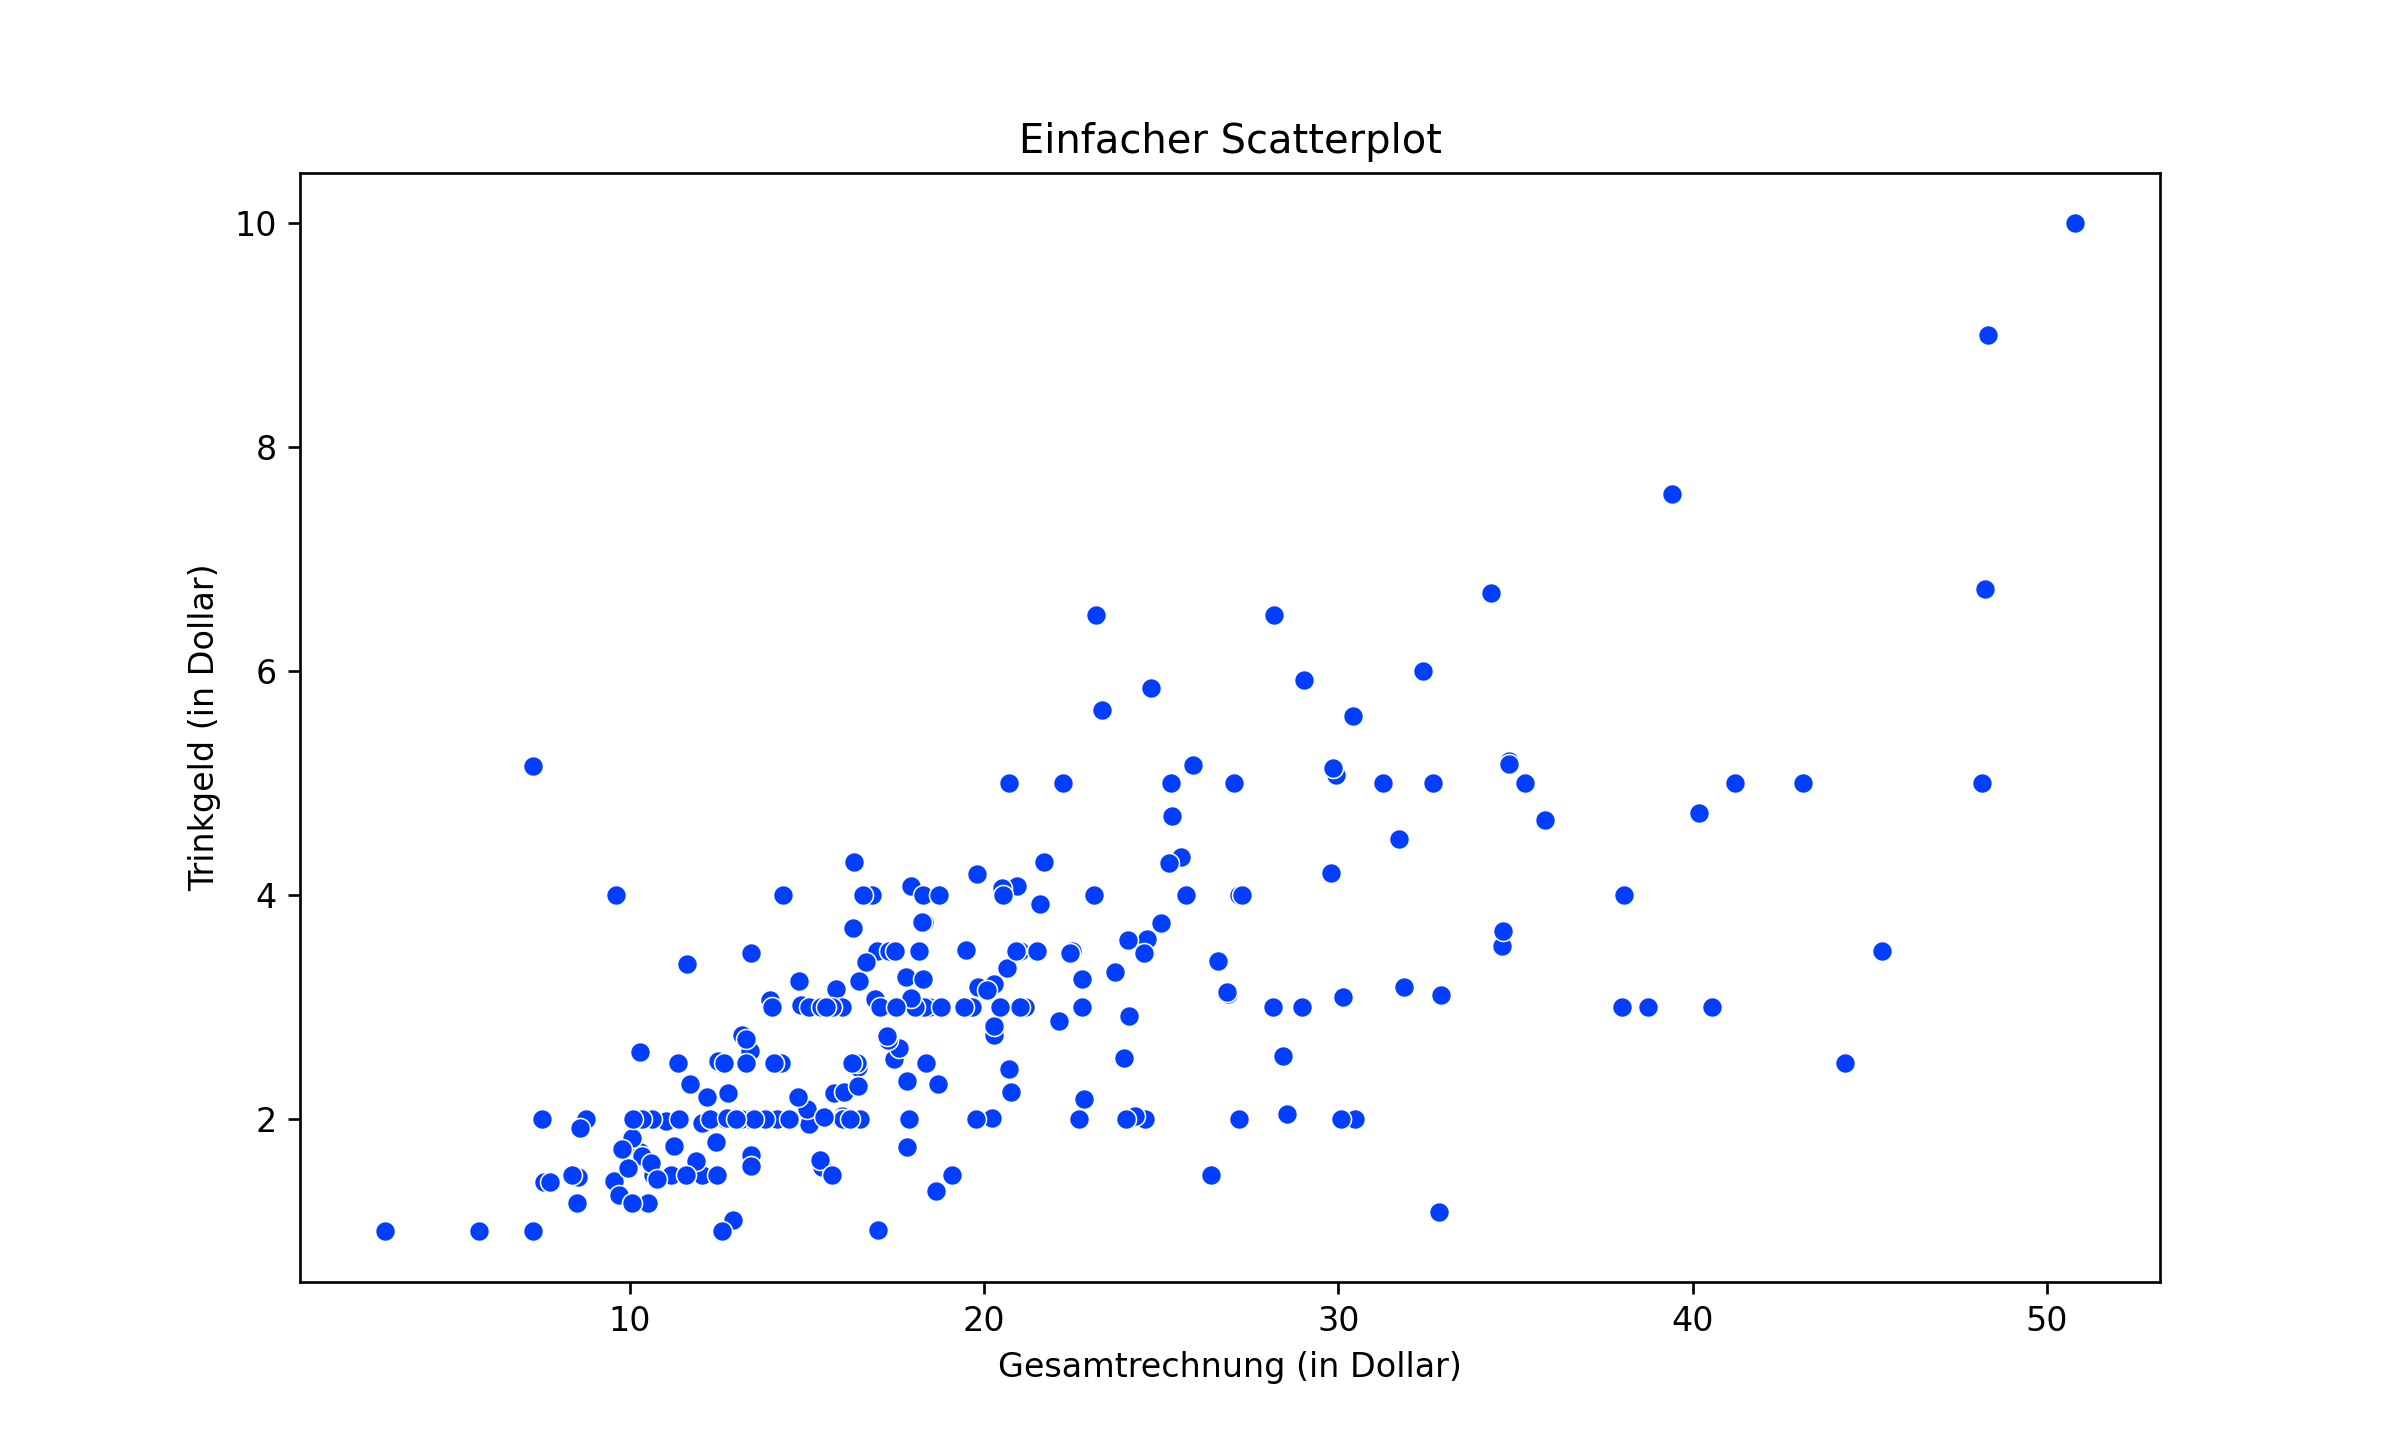
\includegraphics[scale=0.11]{../figures/scatter_plot.png}
        \caption{Simpler Scatterplot }
        \label{fig:scatter_plot}
    \end{figure}
    }
    \only<2>{
    \begin{figure}
        \centering
        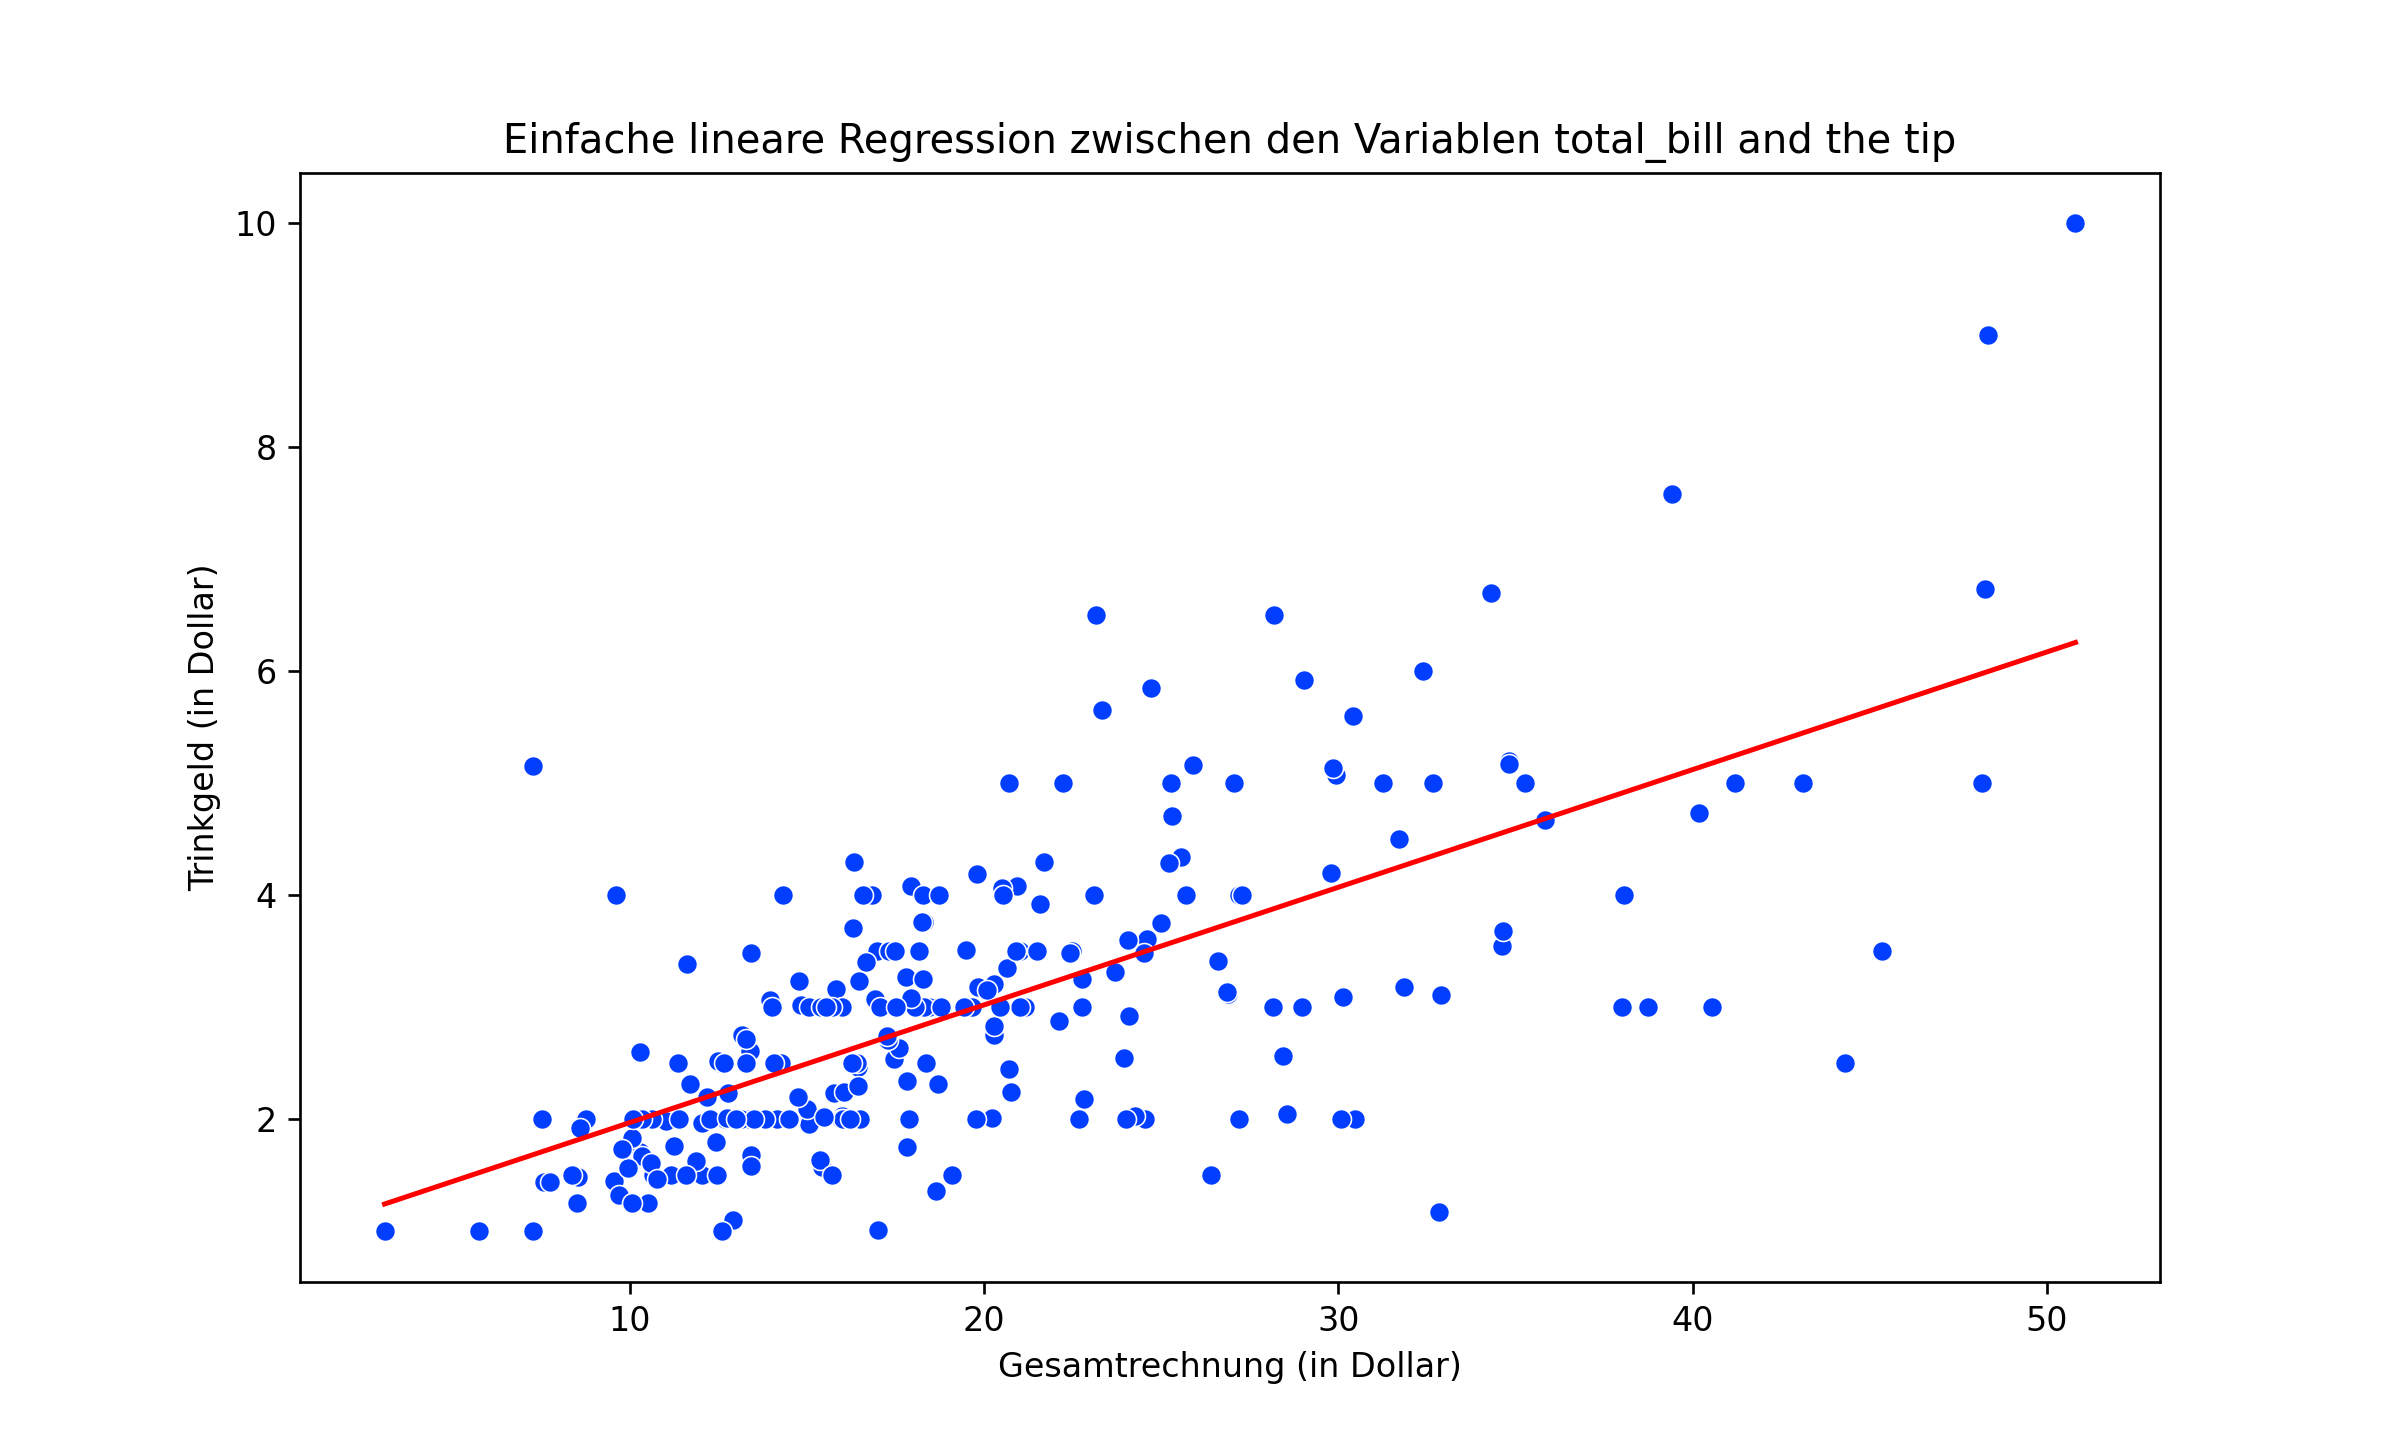
\includegraphics[scale=0.11]{../figures/scatter_plot_regression.png}
        \caption{Simpler Scatterplot mit Regressionsgeraden}
        \label{fig:scatter_plot}
    \end{figure}
    }
    \only<3>{
    \begin{figure}
        \centering
        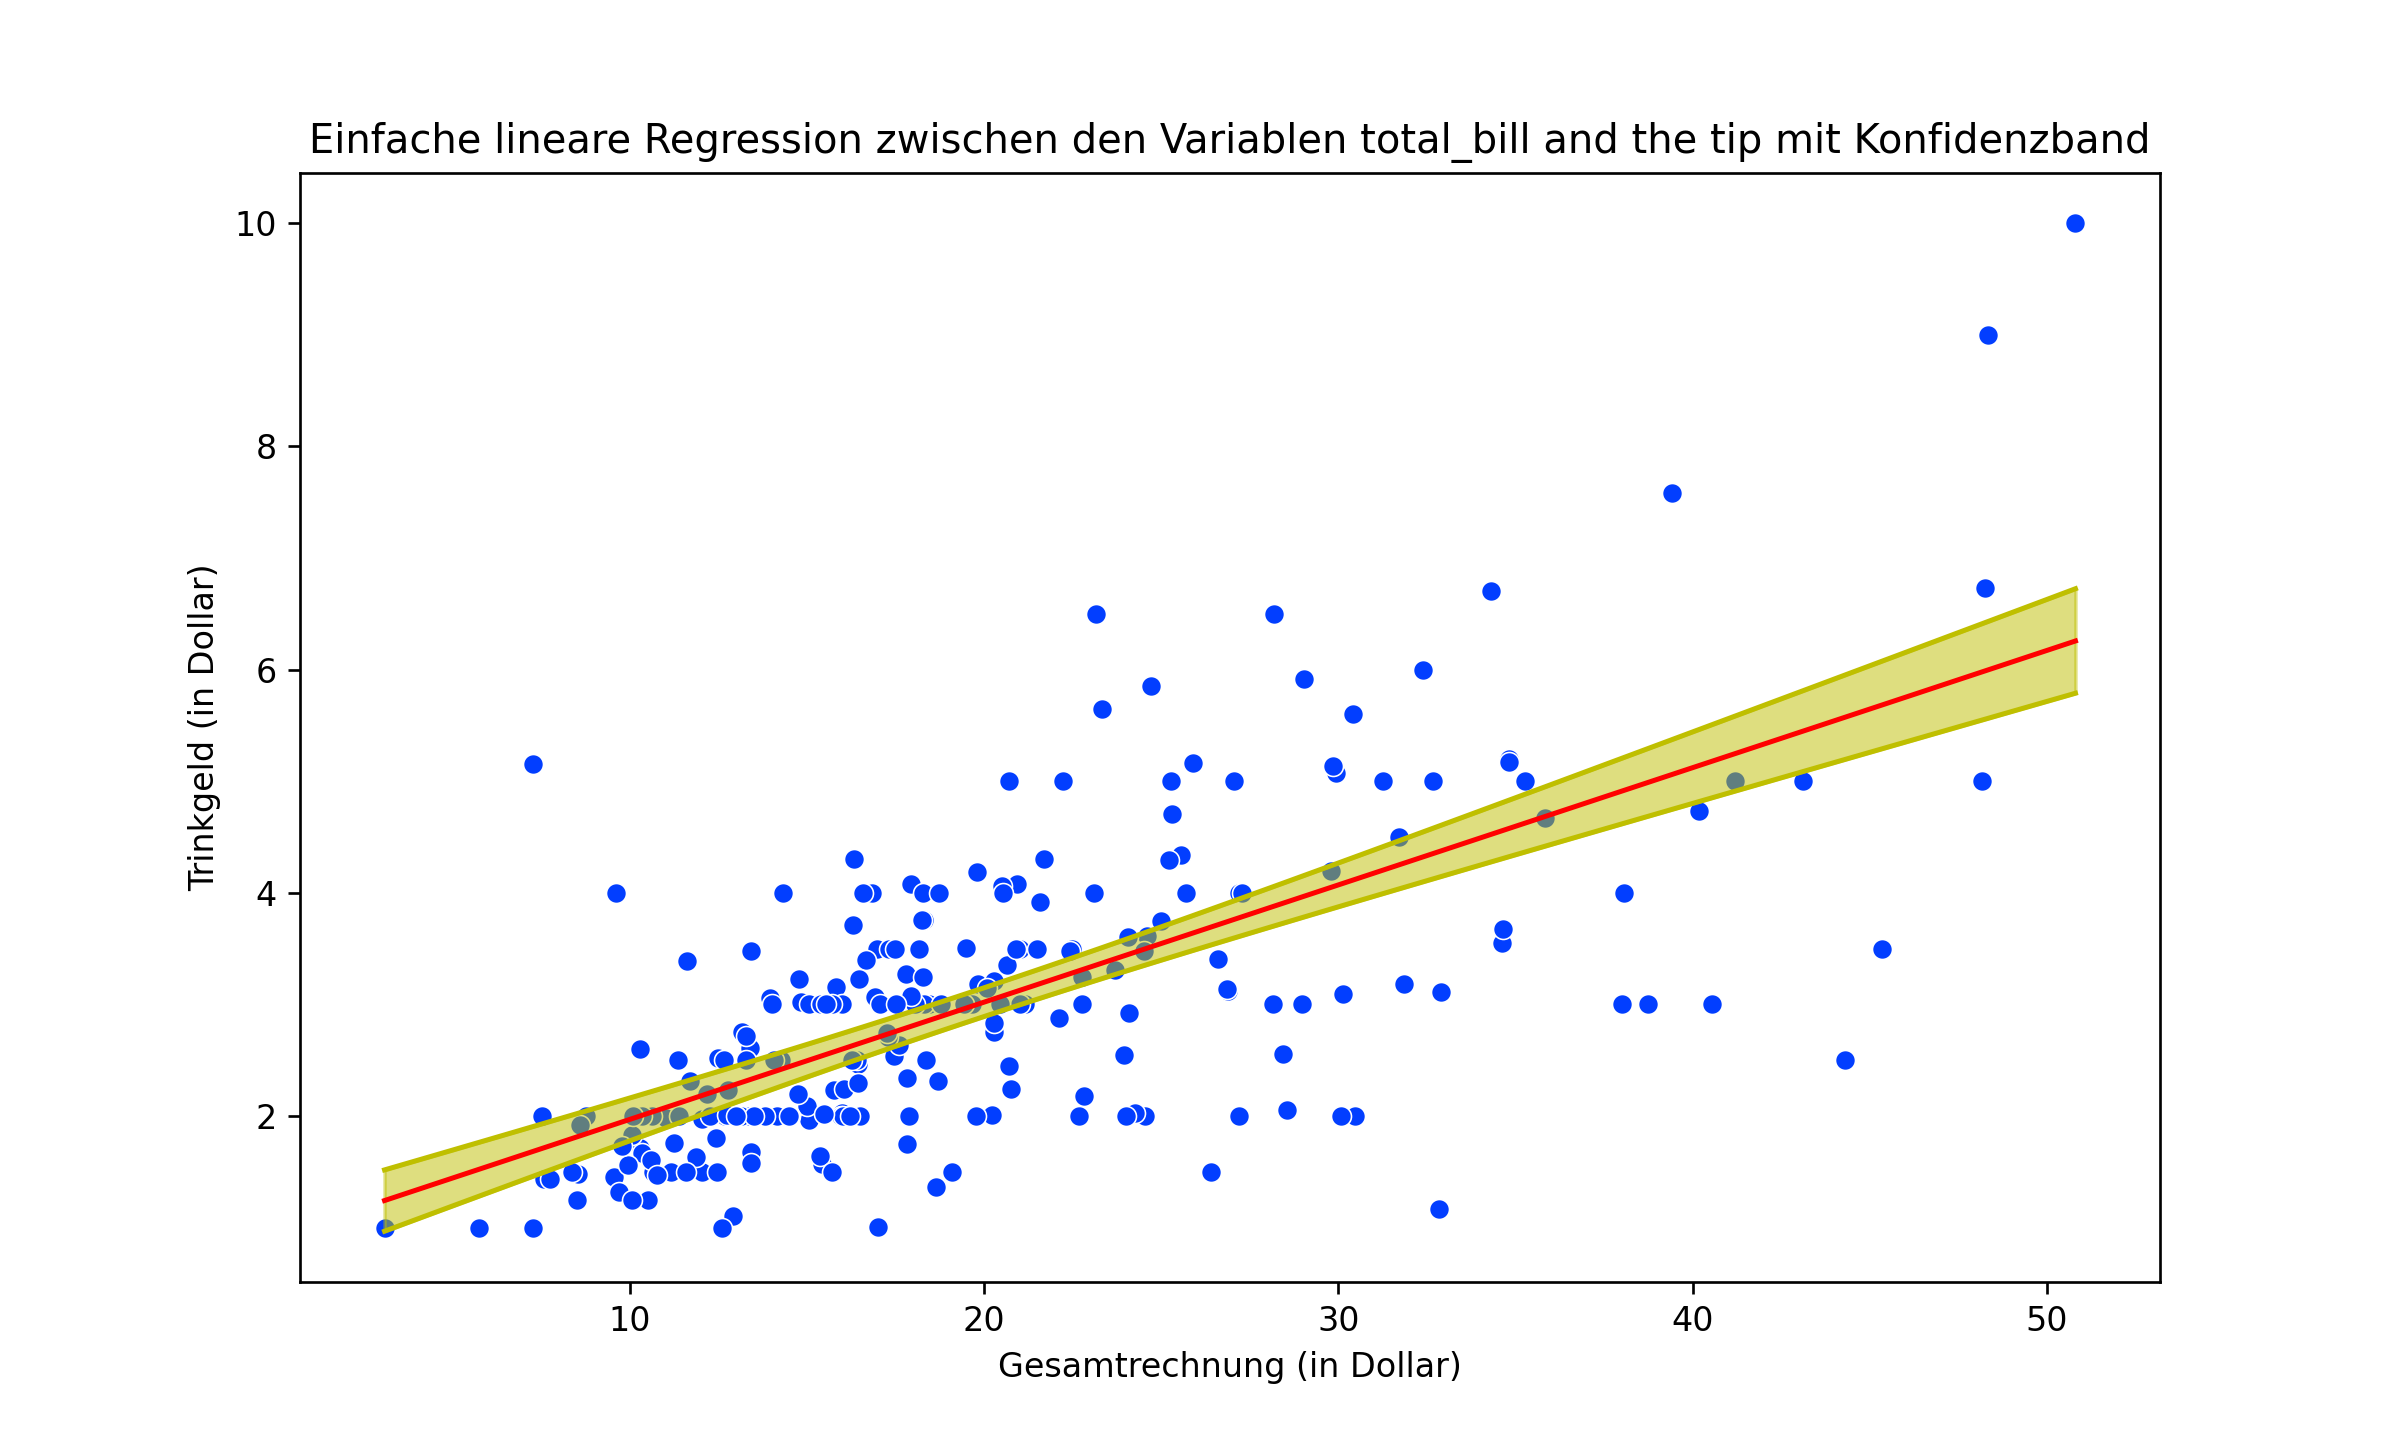
\includegraphics[scale=0.11]{../figures/scatter_plot_confband.png}
        \caption{Simpler Scatterplot mit Regressionsgeraden und Konfidenzband}
        \label{fig:scatter_plot}
    \end{figure}
    }
\end{frame}

\begin{frame}{Lineares Modell}
    Falls eine solcher Zusammenhang gegeben ist spricht man von einem linearen Modell.
    \pause
    \begin{definition}[Lineares Modell]
        Ein $n$-dimensionaler Zufallsvektor $Y$ genügt einem klassischen linearen Modell, falls es eine Darstellung
        \begin{equation}
            Y=\beta_0 + X^\top \beta+\epsilon
        \end{equation}
        mit Erwartungswert $\Ex[\epsilon]=0$ und Kovarianzmatrix $\Sigma_\epsilon=\sigma^2I_n$.\newline
        Gilt zusätzlich $\epsilon\sim\mathcal{N}(0_n, \sigma^2I_n)$, heißt das Modell \textbf{klassisches lineares Modell}.
    \end{definition}
    Dabei nennt man den Vektor $Y=[Y_1, \dots, Y_n]^\top\in\R^n$ Regressand oder abhängige Variable und die Matrix $X=[X_1, \dots, X_n]\in\R^{k\times n}$ Regressor oder unabhängige Variable.
\end{frame}

\begin{frame}{Lineares Modell}
Zur Vereinfachung können wir die Verschiebungskonstante $\beta_0$ und die Steigung $\beta$ zusammenfassen.
Das erlangen wir, indem wir eine $1$ zu dem Vektor der $X_i$ hinzufügen $\tilde{X}_i=(1, X_i)\in\R^{k+1}$.

Dadurch erhalten wir 
$$Y_i= \tilde{\beta}^\top \tilde{X}_i+\epsilon_i,$$
wobei $\epsilon_i\overset{\mathrm{iid}}{\sim}\mathcal{N}(0, \sigma^2)$.
In Matrix Schreibweise ergibt das 
$$Y= \tilde{X}^\top \tilde{\beta}+\epsilon.$$
\end{frame}


\subsection{KQ-Schätzer}
\begin{frame}{KQ-Schätzer}
Sei $\mathcal{D}=\{(X_1,y_1),\dots,(X_n,y_n)\}$ einen Datensatz. Durch die lineare Regression wollen wir den Vektor  $\tilde{\beta}$ schätzen.

Der gleichmäßig beste erwartungstreue Schätzer (UMVU) bei der linearen Regression ist durch den Kleinste-Quadrate-Schätzer gegeben, welcher folgende Gleichung minimiert.

\pause
\begin{equation}
    \hat{\beta} = \argmin_{\tilde{\beta}\in\R^{k+1}}\sum_{i=1}^n\left|y_i-\tilde{\beta}^\top\tilde{X}_i\right|^2
\end{equation}
\end{frame}

\begin{frame}{KQ-Schätzer}
\begin{satz}[KQ-Schätzer in linearen Modellen]\label{stz:kqs}
    Sei $Y = X + \epsilon$ ein lineares Modell
    mit einer $(k + 1)n$-Matrix X und $rg(X) = k + 1$, dann ist für eine beobachtete Realisierung
    $y$ von $Y$ der KQ-Schätzer $\hat{\beta}$ gegeben durch
    $$\hat{\beta}=(\tilde{X}\tilde{X}^\top)^{-1}\tilde{X}Y.$$
    $\hat{\beta}$ ist ein erwartungstreuer Schätzer für $\beta$ mit Kovarianzmatrix $\Sigma_{\hat{\beta}} = \sigma^2(\tilde{X}\tilde{X}^\top)^{-1}$.
\end{satz}
\end{frame}
\begin{frame}{Beweis von Satz \ref{stz:kqs}}
    \begin{proof}
        \dots
    \end{proof}
\end{frame}

\begin{frame}{Implementierung des KQ-Schätzers}
Die Darstellung des KQ-Schätzers aus Satz \ref{stz:kqs} haben wir verwendet, um den Schätzer für $\tilde{\beta}$ zu implementieren.
\pause
\lstinputlisting[language=Python, caption=Simple lineare Regression aus der Datei \lstinline{regression.py}, firstline=34, lastline=44, firstnumber=34, label=lst:umvubeta]{../code/regression.py}
\end{frame}

\begin{frame}{Statistik der linearen Regression}
\scriptsize
\begin{table}[]
    \begin{center}
\begin{tabular}{lclc}
\toprule
\textbf{Dep. Variable:}    &       tip        & \textbf{  R-squared:         } &     0.457   \\
\textbf{Model:}            &       OLS        & \textbf{  Adj. R-squared:    } &     0.454   \\
\textbf{Method:}           &  Least Squares   & \textbf{  F-statistic:       } &     203.4   \\
\textbf{Date:}             & Wed, 30 Aug 2023 & \textbf{  Prob (F-statistic):} &  6.69e-34   \\
\textbf{Time:}             &     15:50:13     & \textbf{  Log-Likelihood:    } &   -350.54   \\
\textbf{No. Observations:} &         244      & \textbf{  AIC:               } &     705.1   \\
\textbf{Df Residuals:}     &         242      & \textbf{  BIC:               } &     712.1   \\
\textbf{Df Model:}         &           1      & \textbf{                     } &             \\
\textbf{Covariance Type:}  &    nonrobust     & \textbf{                     } &             \\
\bottomrule
\end{tabular}
\begin{tabular}{lcccccc}
               & \textbf{coef} & \textbf{std err} & \textbf{t} & \textbf{P$> |$t$|$} & \textbf{[0.025} & \textbf{0.975]}  \\
\midrule
\textbf{const} &       0.9203  &        0.160     &     5.761  &         0.000        &        0.606    &        1.235     \\
\textbf{x1}    &       0.1050  &        0.007     &    14.260  &         0.000        &        0.091    &        0.120     \\
\bottomrule
\end{tabular}
\begin{tabular}{lclc}
\textbf{Omnibus:}       & 20.185 & \textbf{  Durbin-Watson:     } &    2.151  \\
\textbf{Prob(Omnibus):} &  0.000 & \textbf{  Jarque-Bera (JB):  } &   37.750  \\
\textbf{Skew:}          &  0.443 & \textbf{  Prob(JB):          } & 6.35e-09  \\
\textbf{Kurtosis:}      &  4.711 & \textbf{  Cond. No.          } &     53.0  \\
\bottomrule
\end{tabular}
%\caption{OLS Regression Results}
\end{center}

Notes: \newline
 [1] Standard Errors assume that the covariance matrix of the errors is correctly specified.
    \caption{ Zusammenfassung der OLS Regressions Statistik.}
    \label{tab:regression}
\end{table} 
\end{frame}

\begin{frame}{Darstellung der linearen Regression}
\begin{figure}
    \centering
    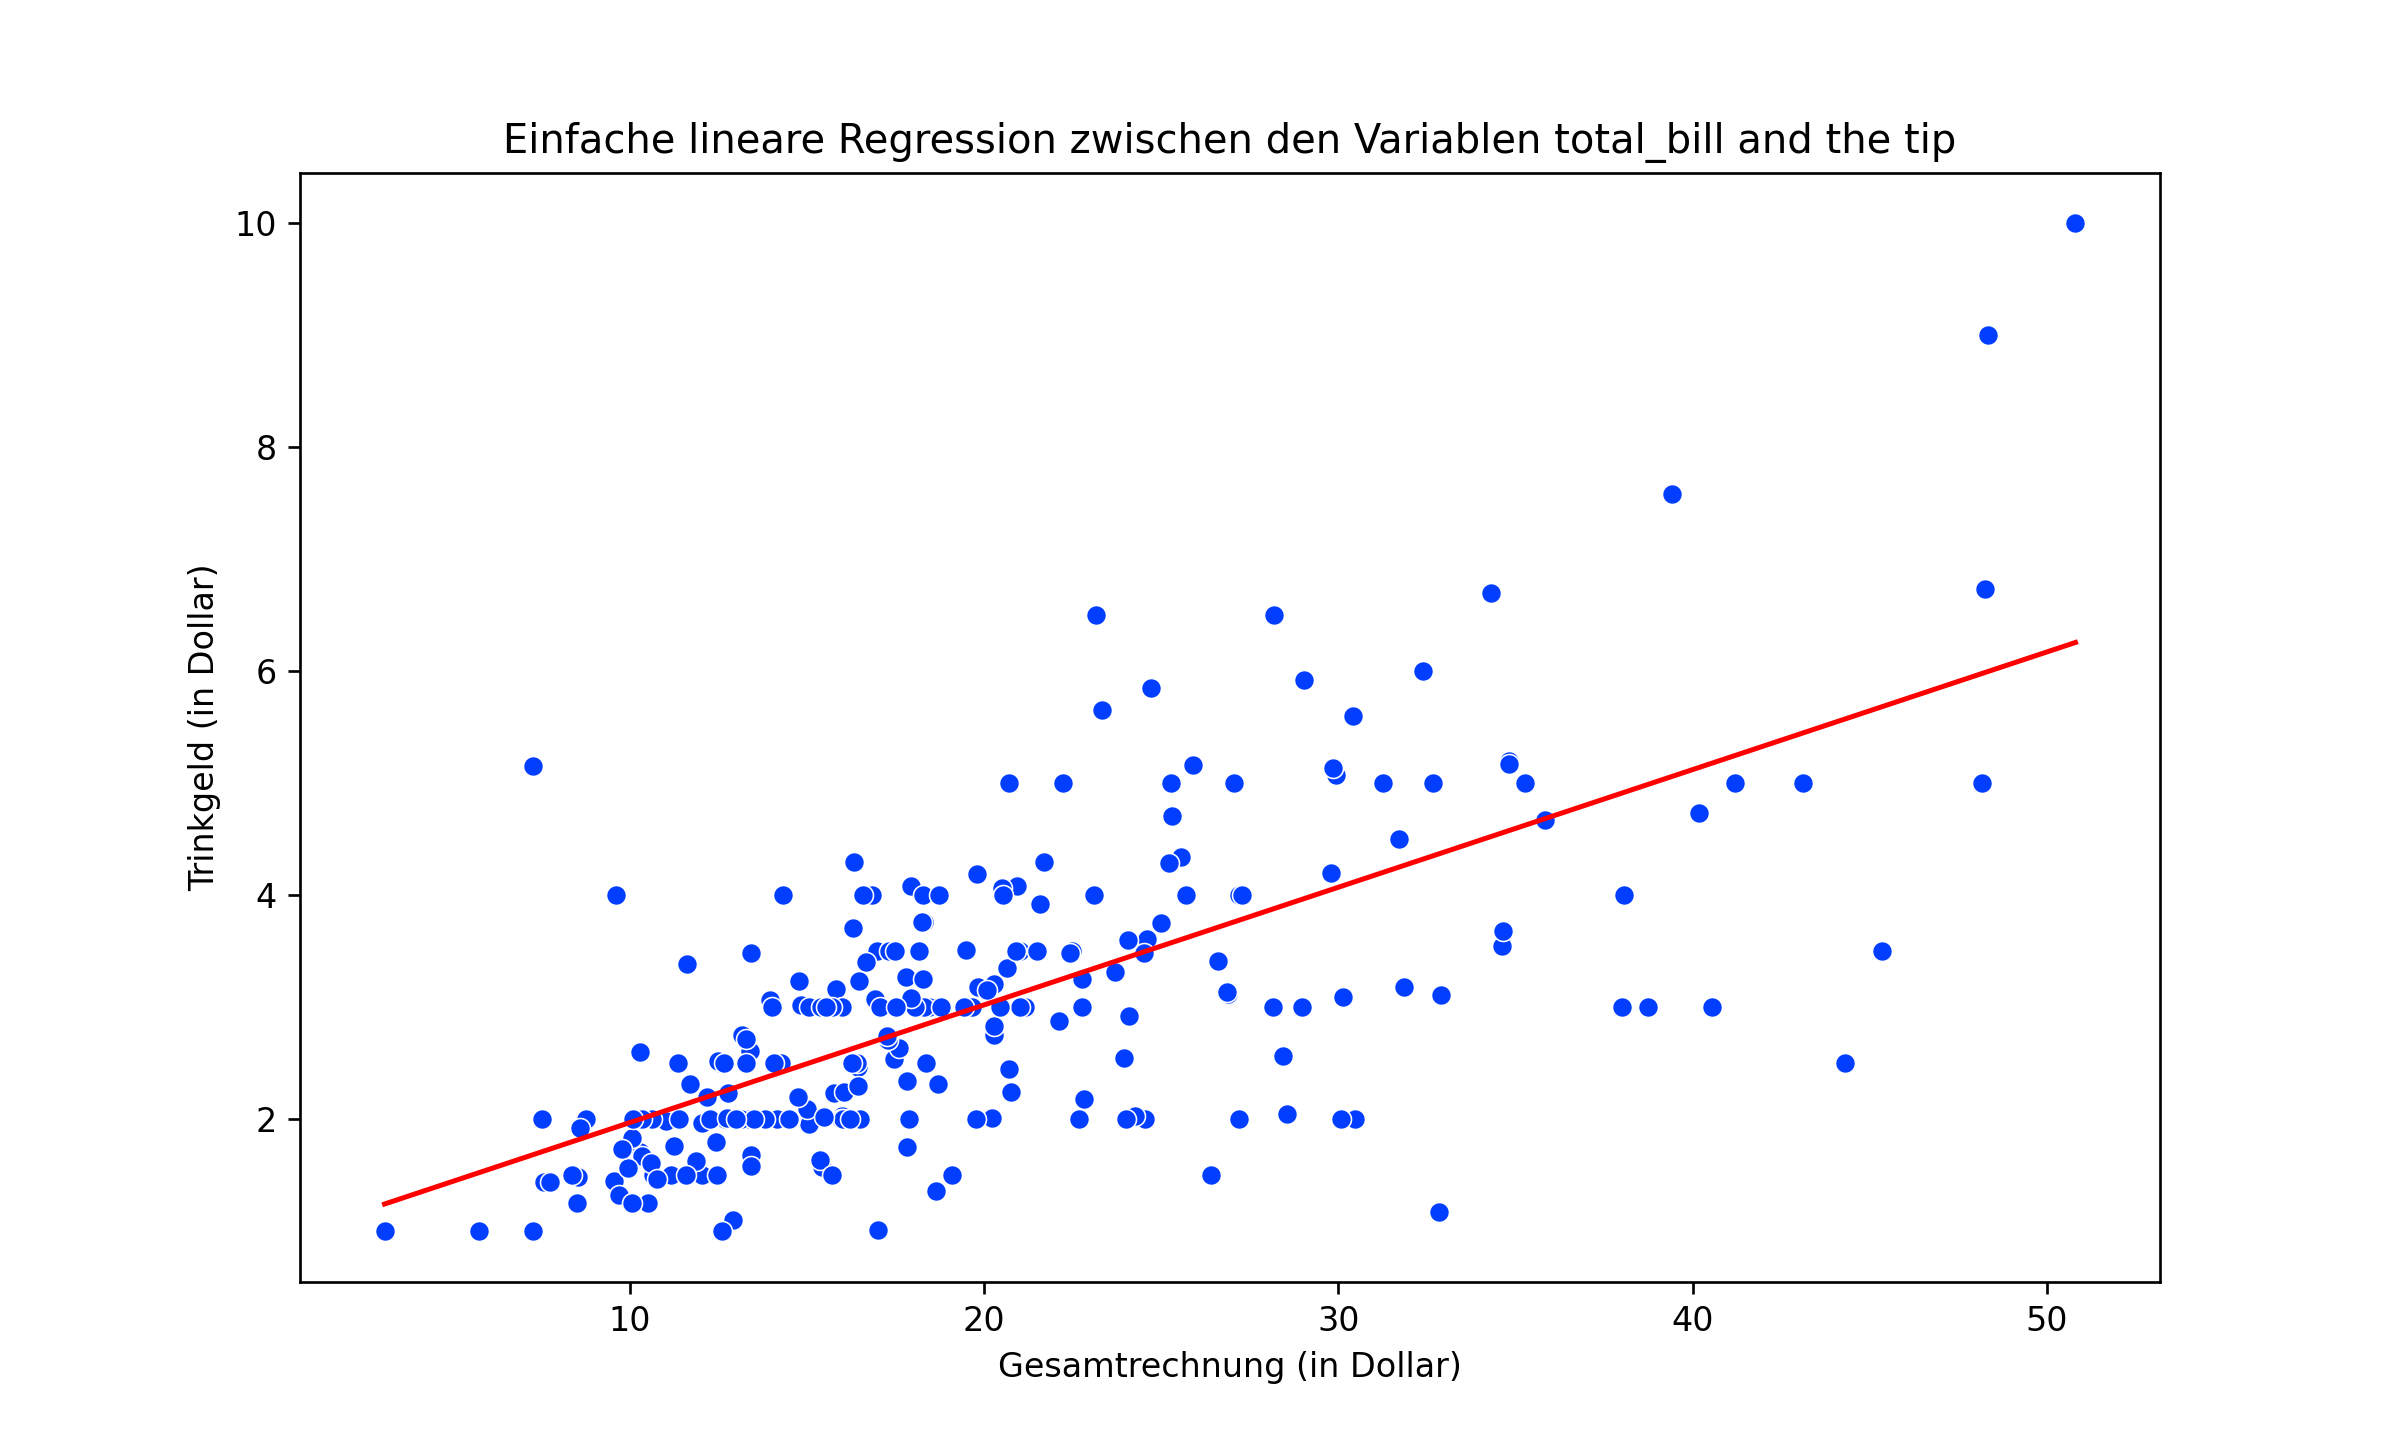
\includegraphics[scale=0.13]{../../paper/figures/simple_reg.png}
    \caption{In einen Scatterplot eingezeichnete selbstimplementierte Regressionsgerade.}
    \label{fig:regression}
\end{figure}
\end{frame}

\subsection{p-Wert}
\begin{frame}{p-Wert}
    \dots
\end{frame}

\subsection{Konfidenzband für eine Lineare Regression}
\begin{frame}{Konfidenzband für eine Lineare Regression}
    
    \dots
\end{frame}
